\documentclass[11pt, a4paper]{article}
\usepackage{pdfpages}
\usepackage{parallel}
\usepackage[T2A]{fontenc}
\usepackage{ucs}
\usepackage[utf8x]{inputenc}
\usepackage[polish,english,russian]{babel}
\usepackage{hyperref}
\usepackage{rotating}
\usepackage[inner=2cm,top=1.8cm,outer=2cm,bottom=2.3cm,nohead]{geometry}
\usepackage{listings}
\usepackage{graphicx}
\usepackage{wrapfig}
\usepackage{longtable}
\usepackage{indentfirst}
\usepackage{array}
\usepackage{tikzsymbols}
\usepackage{soul}
\usepackage[ruled,vlined]{algorithm2e}
%\counterwithout{figure}{section} 

\usepackage{url}
\makeatletter
\g@addto@macro{\UrlBreaks}{\UrlOrds}
\makeatother

\newcolumntype{P}[1]{>{\raggedright\arraybackslash}p{#1}}
\frenchspacing
\usepackage{fixltx2e} %text sub- and superscripts
\usepackage{icomma} % коскі ў матэматычным рэжыме
\PreloadUnicodePage{4}

\newcommand{\longpage}{\enlargethispage{\baselineskip}}
\newcommand{\shortpage}{\enlargethispage{-\baselineskip}}

\def\switchlang#1{\expandafter\csname switchlang#1\endcsname}
\def\switchlangbe{
\let\saverefname=\refname%
\def\refname{Літаратура}%
\def\figurename{Іл.}%
}
\def\switchlangen{
\let\saverefname=\refname%
\def\refname{References}%
\def\figurename{Fig.}%
}
\def\switchlangru{
\let\saverefname=\refname%
\let\savefigurename=\figurename%
\def\refname{Литература}%
\def\figurename{Рис.}%
}

\hyphenation{admi-ni-stra-tive}
\hyphenation{ex-pe-ri-ence}
\hyphenation{fle-xi-bi-li-ty}
\hyphenation{Py-thon}
\hyphenation{ma-the-ma-ti-cal}
\hyphenation{re-ported}
\hyphenation{imp-le-menta-tions}
\hyphenation{pro-vides}
\hyphenation{en-gi-neering}
\hyphenation{com-pa-ti-bi-li-ty}
\hyphenation{im-pos-sible}
\hyphenation{desk-top}
\hyphenation{elec-tro-nic}
\hyphenation{com-pa-ny}
\hyphenation{de-ve-lop-ment}
\hyphenation{de-ve-loping}
\hyphenation{de-ve-lop}
\hyphenation{da-ta-ba-se}
\hyphenation{plat-forms}
\hyphenation{or-ga-ni-za-tion}
\hyphenation{pro-gramming}
\hyphenation{in-stru-ments}
\hyphenation{Li-nux}
\hyphenation{sour-ce}
\hyphenation{en-vi-ron-ment}
\hyphenation{Te-le-pathy}
\hyphenation{Li-nux-ov-ka}
\hyphenation{Open-BSD}
\hyphenation{Free-BSD}
\hyphenation{men-ti-on-ed}
\hyphenation{app-li-ca-tion}

\def\progref!#1!{\texttt{#1}}
\renewcommand{\arraystretch}{2} %Іначай формулы ў матрыцы зліпаюцца з лініямі
\usepackage{array}

\def\interview #1 (#2), #3, #4, #5\par{

\section[#1, #3, #4]{#1 -- #3, #4}
\def\qname{LVEE}
\def\aname{#1}
\def\q ##1\par{{\noindent \bf \qname: ##1 }\par}
\def\a{{\noindent \bf \aname: } \def\qname{L}\def\aname{#2}}
}

\def\interview* #1 (#2), #3, #4, #5\par{

\section*{#1\\{\small\rm #3, #4. #5}}
\ifx\ParallelWhichBox\undefined%
    \addcontentsline{toc}{section}{#1, #3, #4}%
\else%
\ifnum\ParallelWhichBox=0%
    \addcontentsline{toc}{section}{#1, #3, #4}%
\fi\fi%

\def\qname{LVEE}
\def\aname{#1}
\def\q ##1\par{{\noindent \bf \qname: ##1 }\par}
\def\a{{\noindent \bf \aname: } \def\qname{L}\def\aname{#2}}
}

\newcommand{\interviewfooter}[1]{
\vskip 1em
\noindent \textit{#1}
}

\switchlang{en}
\begin{document}

\title{1989 "--- Prohance PowerMouse}
\date{}
\maketitle
\selectlanguage{english}
The Prohance Mouse was released by Prohance Technologies inc. in 1989 as part of a family of several mice and one trackball designed for use with Lotus 1-2-3 spreadsheets (and some other similar applications). The concept of Prohance is to place a lot of additional buttons on the body, which, according to the developers, save the user from frequently moving his hand from the mouse to the keyboard and vice versa. The Prohance mouse contains an additional functional keyboard on the front part of the case. This model, named PowerMouse 50 on its box, has 10 function buttons (figure \ref{fig:ProhancePhoto}), and in general their number could reach up to 40 (which was implemented due to a very elongated mouse body, similar to a TV remote control) \cite{livingston}.

\begin{figure}[h]
    \centering
    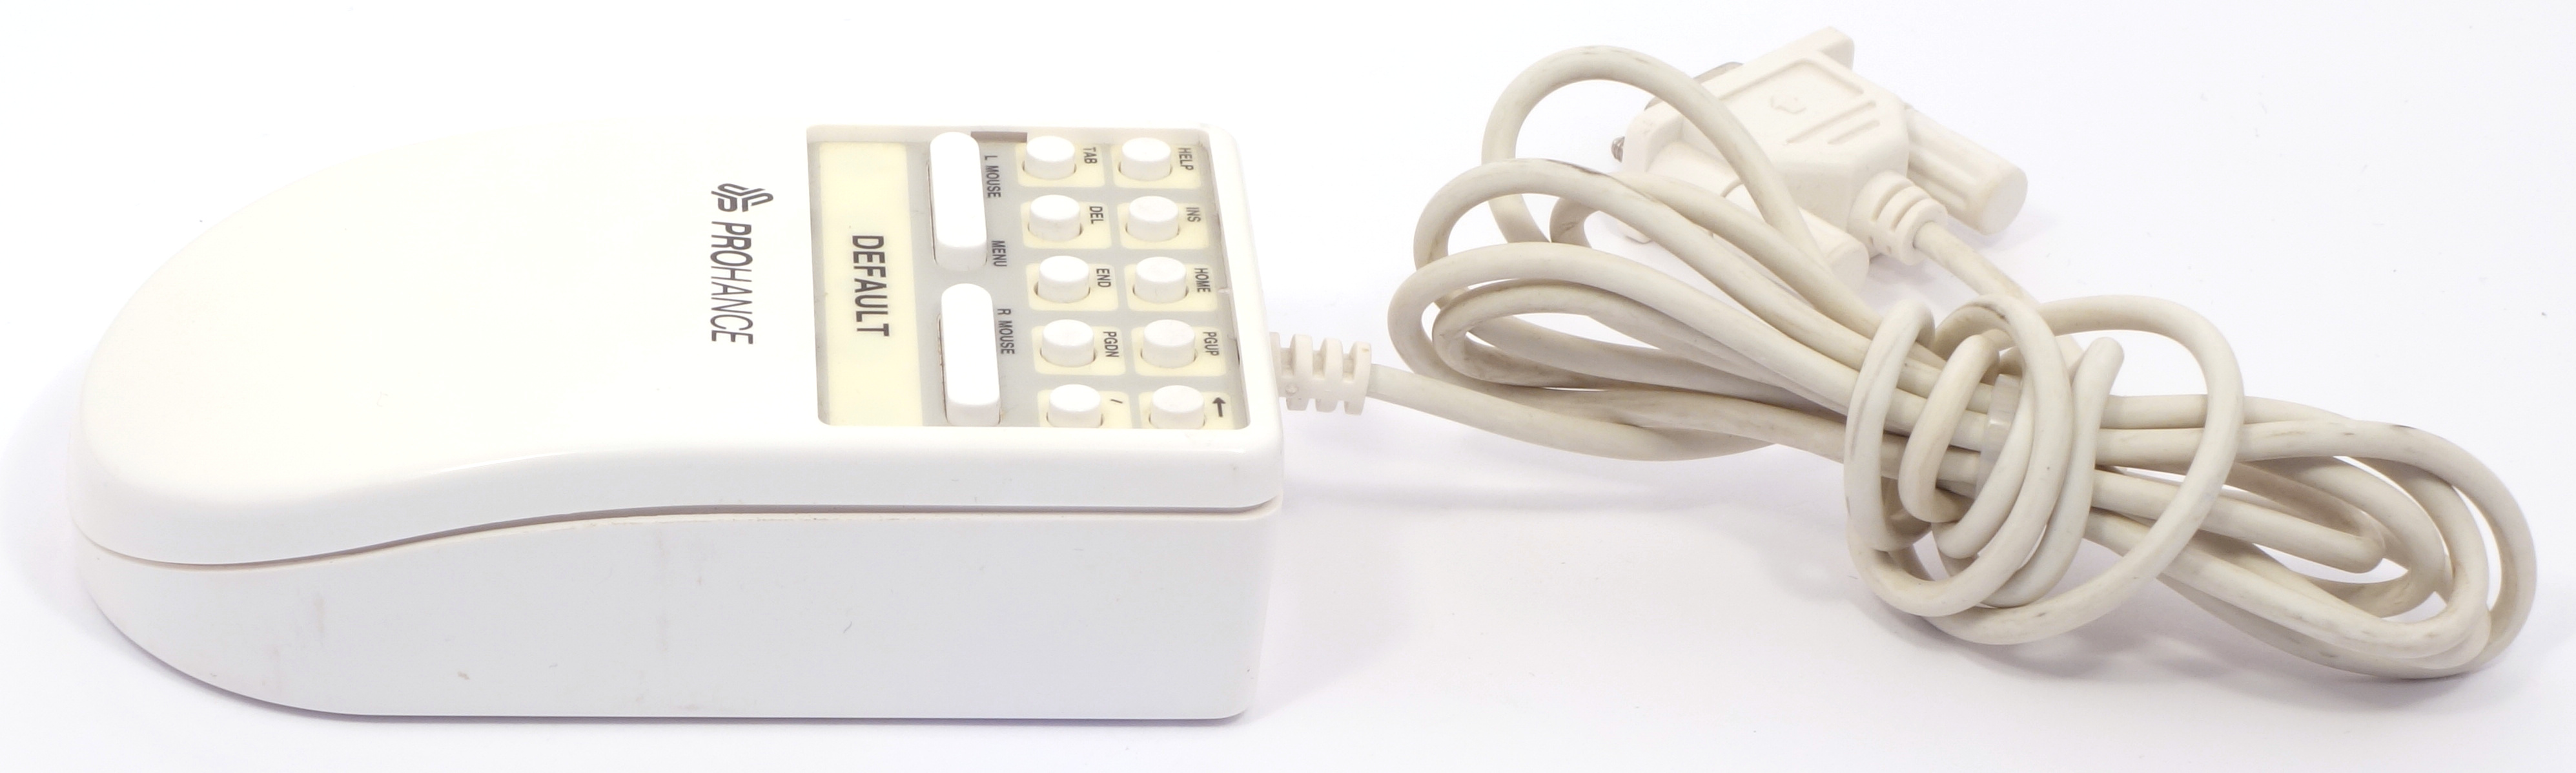
\includegraphics[scale=0.55]{1989_prohance_powermouse/pic_30.jpg}
    \caption{Prohance PowerMouse}
    \label{fig:ProhancePhoto}
\end{figure}

When working with Lotus 1-2-3 spreadsheets, each function key of this mouse corresponds to a certain sequence of keycodes, that is, in fact, pressing a function button executes a given macro command. Otherwise, this pointing device acts like any other mouse, allowing you to use it with any graphics software.

In terms of ergonomics, the case of this device repeats the shape of the Dove Bar Microsoft mouse, which, in turn, borrowed the shape from the grinding bar, and therefore turned out to be one of the first ergonomic mice (figure \ref{fig:ProhanceSize}).

\begin{figure}[h]
    \centering
    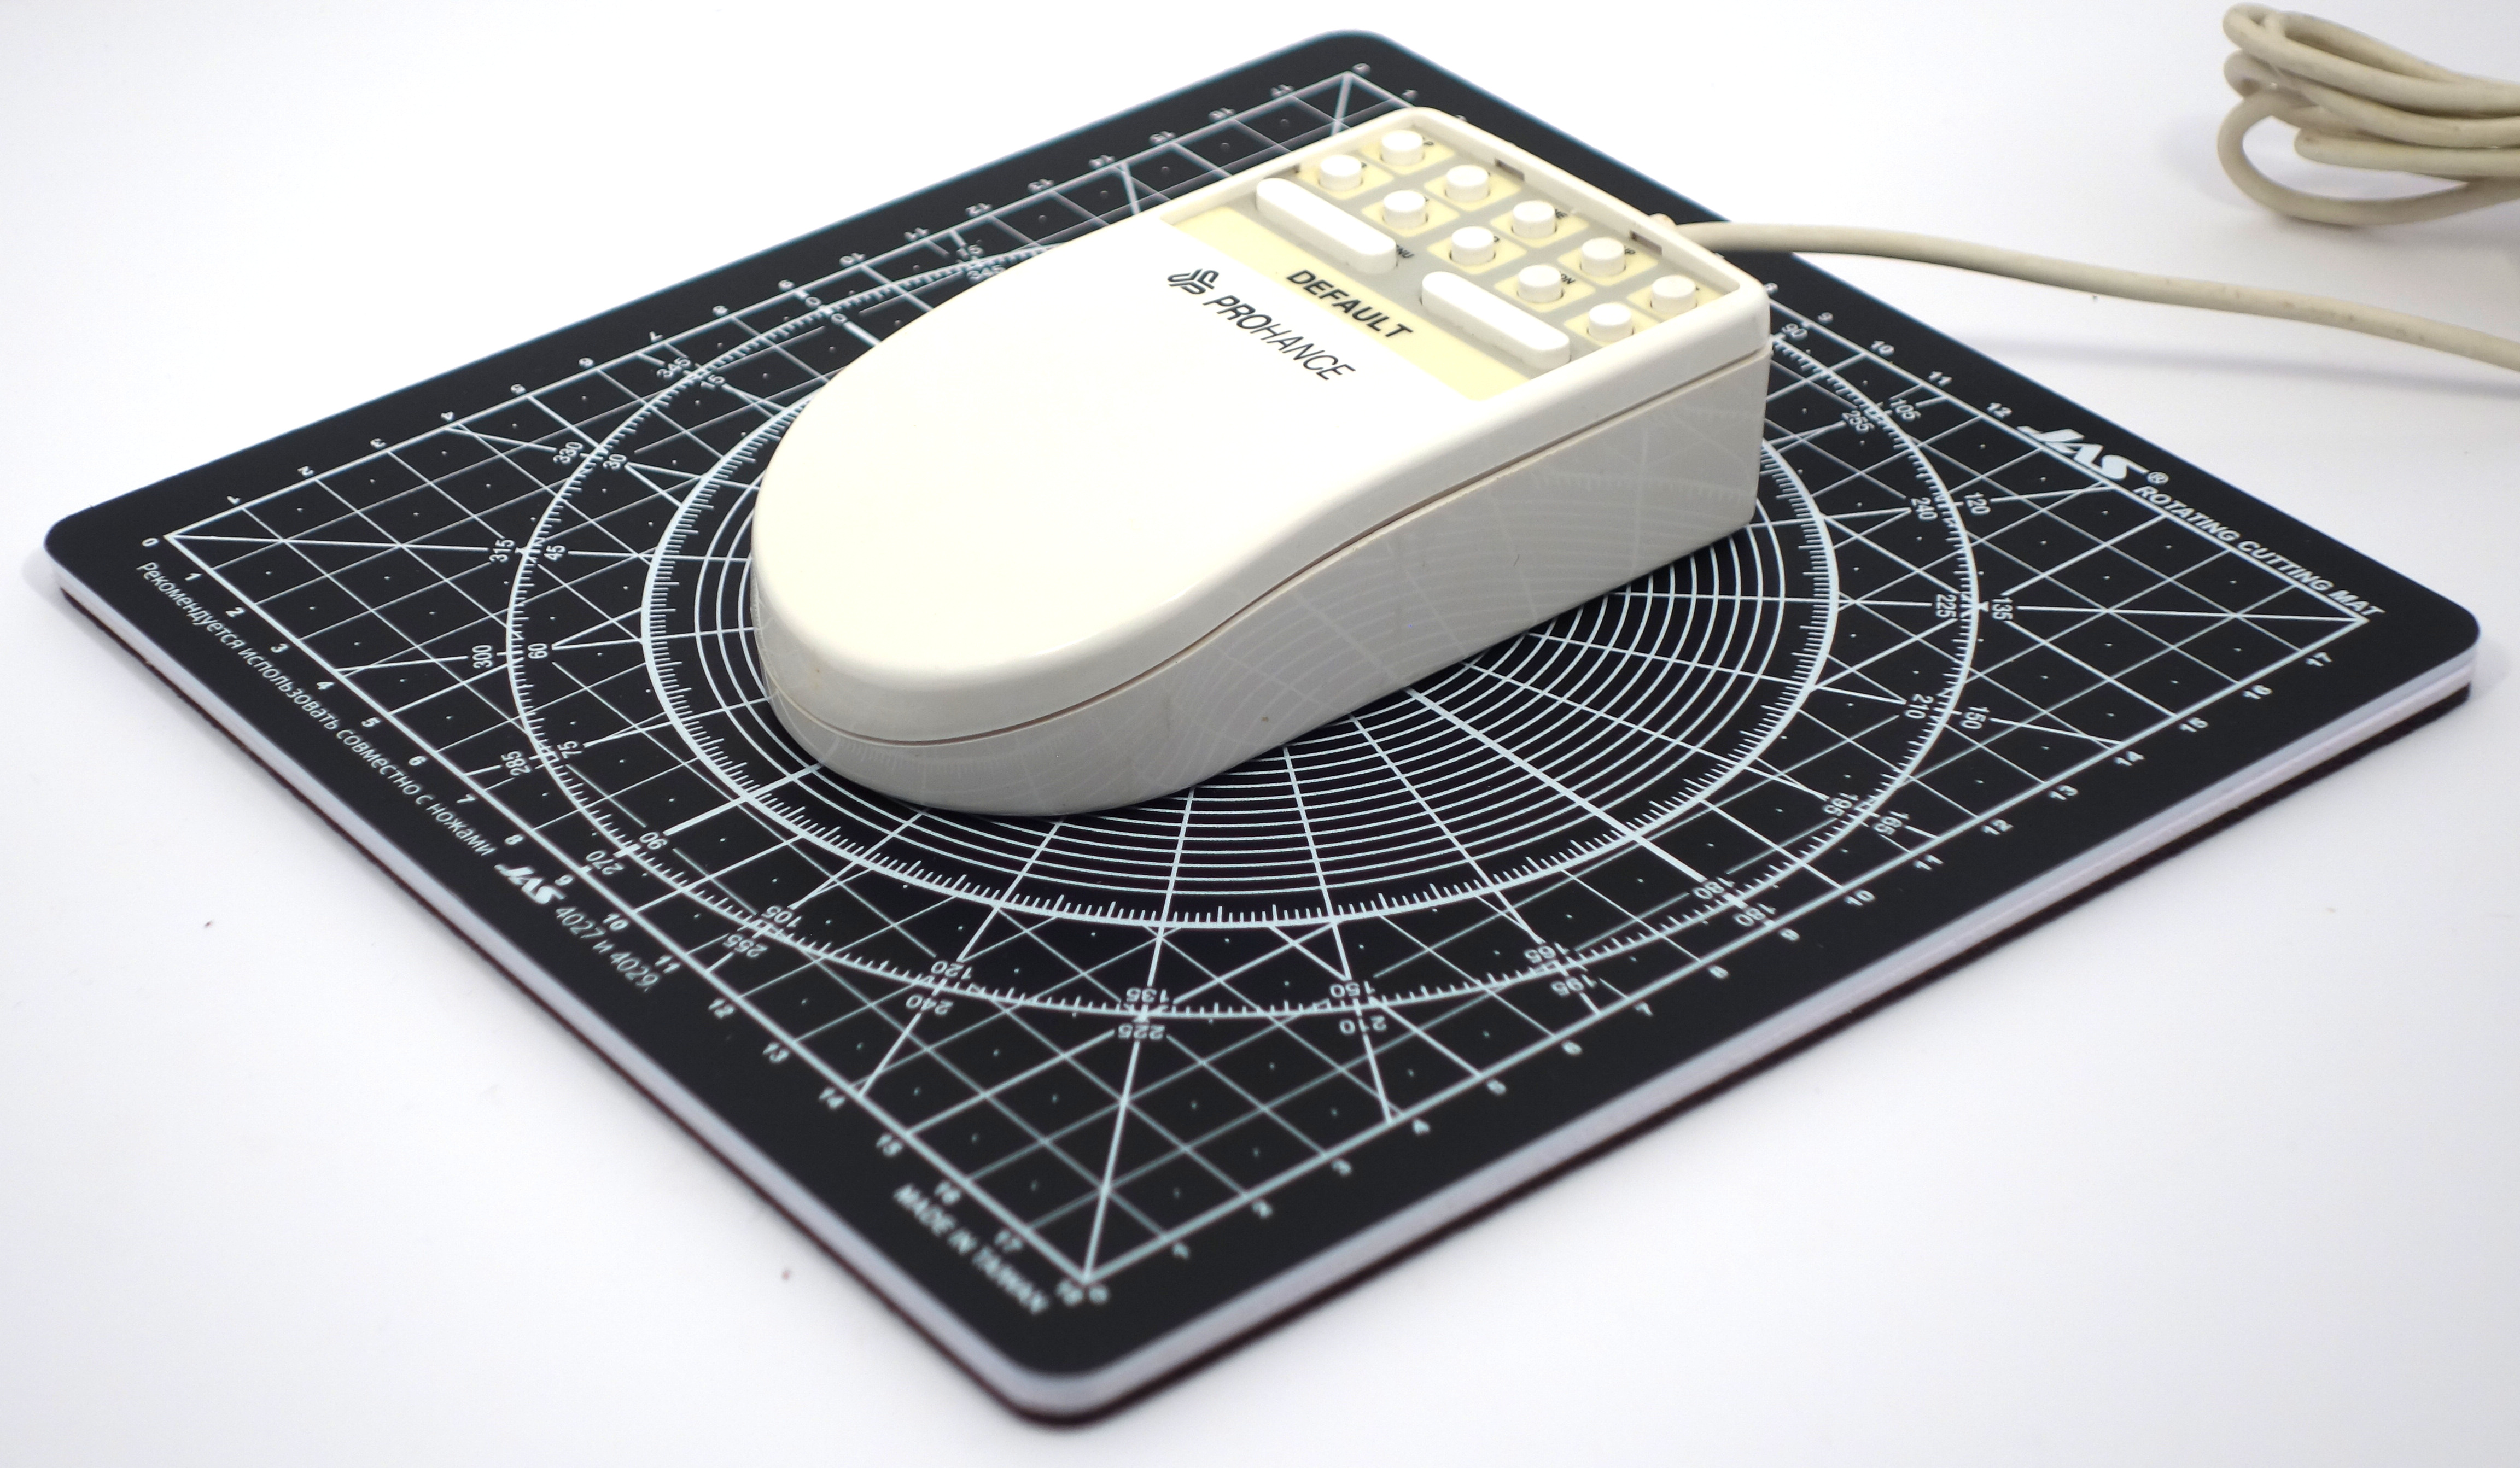
\includegraphics[scale=0.35]{1989_prohance_powermouse/size_30.jpg}
    \caption{Prohance Mouse on a graduated pad with a grid step of 1~cm}
    \label{fig:ProhanceSize}
\end{figure}

Therefore, the shape of the Prohance PoverMouse has no flaws in ergonomics (unlike its fellow PowerMouse 100 with a long body carrying forty function keys). However, an important drawback is the size of the keys: both the main buttons and the additional Prohance keys have a very small area, which makes them much worse than the buttons of a similarly shaped Microsoft mouse. The keycaps are made of rubber, like the buttons of a pocket calculator, but they make a barely audible click when pressed. At the same time, the key travel is rather big, so the probability of accidentally pressing a key is small.

Keycaps have no tactile or visual distinguishing features. This is especially problematic for function keys: they have round caps of the same size, so you need to carefully monitor the correct position of your finger before pressing. To identify the keys, replaceable inserts are provided - overlays placed over the functional keyboard. However, due to the size of the mouse, the labels on them are small, fingers overlap them, and an untrained user has to look closely to find the right one (the difference in the size of the fingertip and the function button is clearly visible in figure \ref{fig:ProhanceHand}).

\begin{figure}[h]
    \centering
    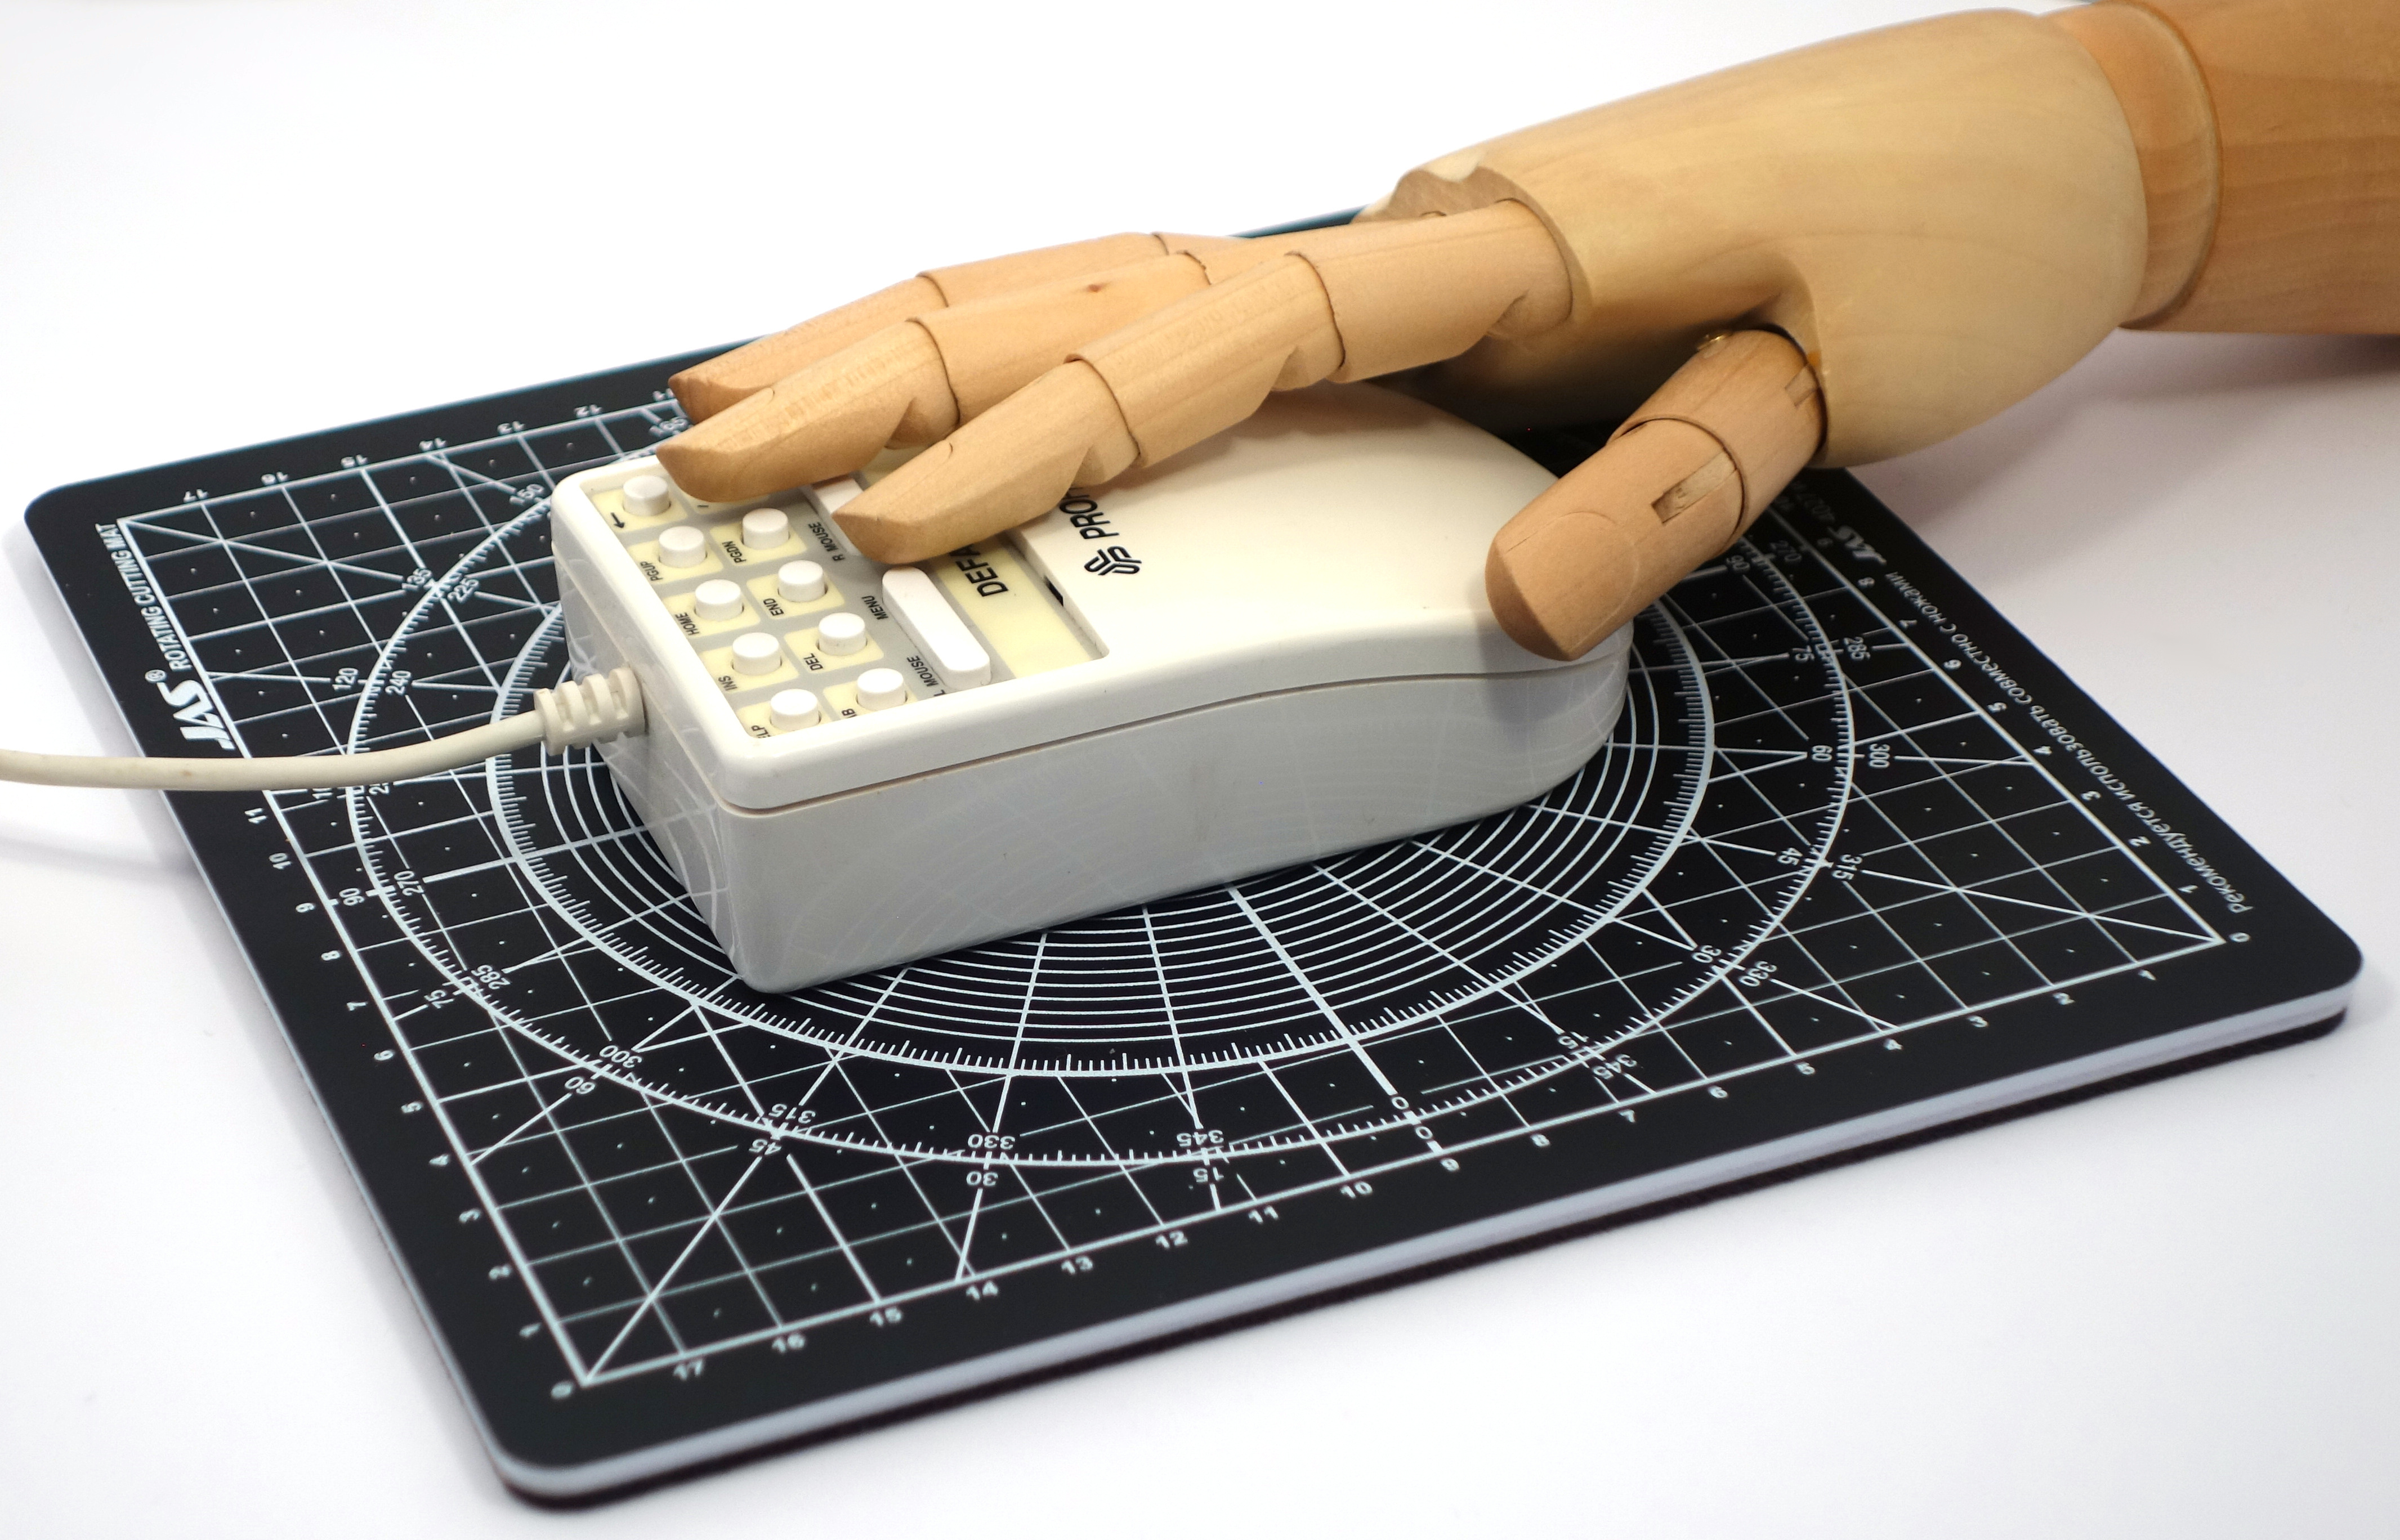
\includegraphics[scale=0.35]{1989_prohance_powermouse/hand_30.jpg}
    \caption{Prohance Mouse with a human hand model}
    \label{fig:ProhanceHand}
\end{figure}

Therefore, in general, the Prohance PowerMouse received negative feedback from users who were forced to click on the extremely narrow left and right mouse buttons, and peer at the small labels between the rows of function keys.

As \cite{prohance} notes, the earlier version of the driver contained errors that caused the mouse to work inadequately in Microsoft Word (even its slight movement led to page scrolling), which were fixed in the updated version. There was also some software incompatibility with the Microsoft mouse driver, which resulted in the mouse not working with some applications.

At the same time, setting up Prohance through the bundled software is quite simple. Unlike other mice of the time, the Prohance does not have software-based on-screen menus - instead, function key remapping is suggested to be used. Prohance provides a macro recording feature that allows you to define new templates for its function keys as well as modify existing ones.
The driver also allows the user to adjust the mouse sensitivity level via the configuration file, however dynamic regulation of mouse acceleration has not been implemented.

\begin{figure}[h]
    \centering
    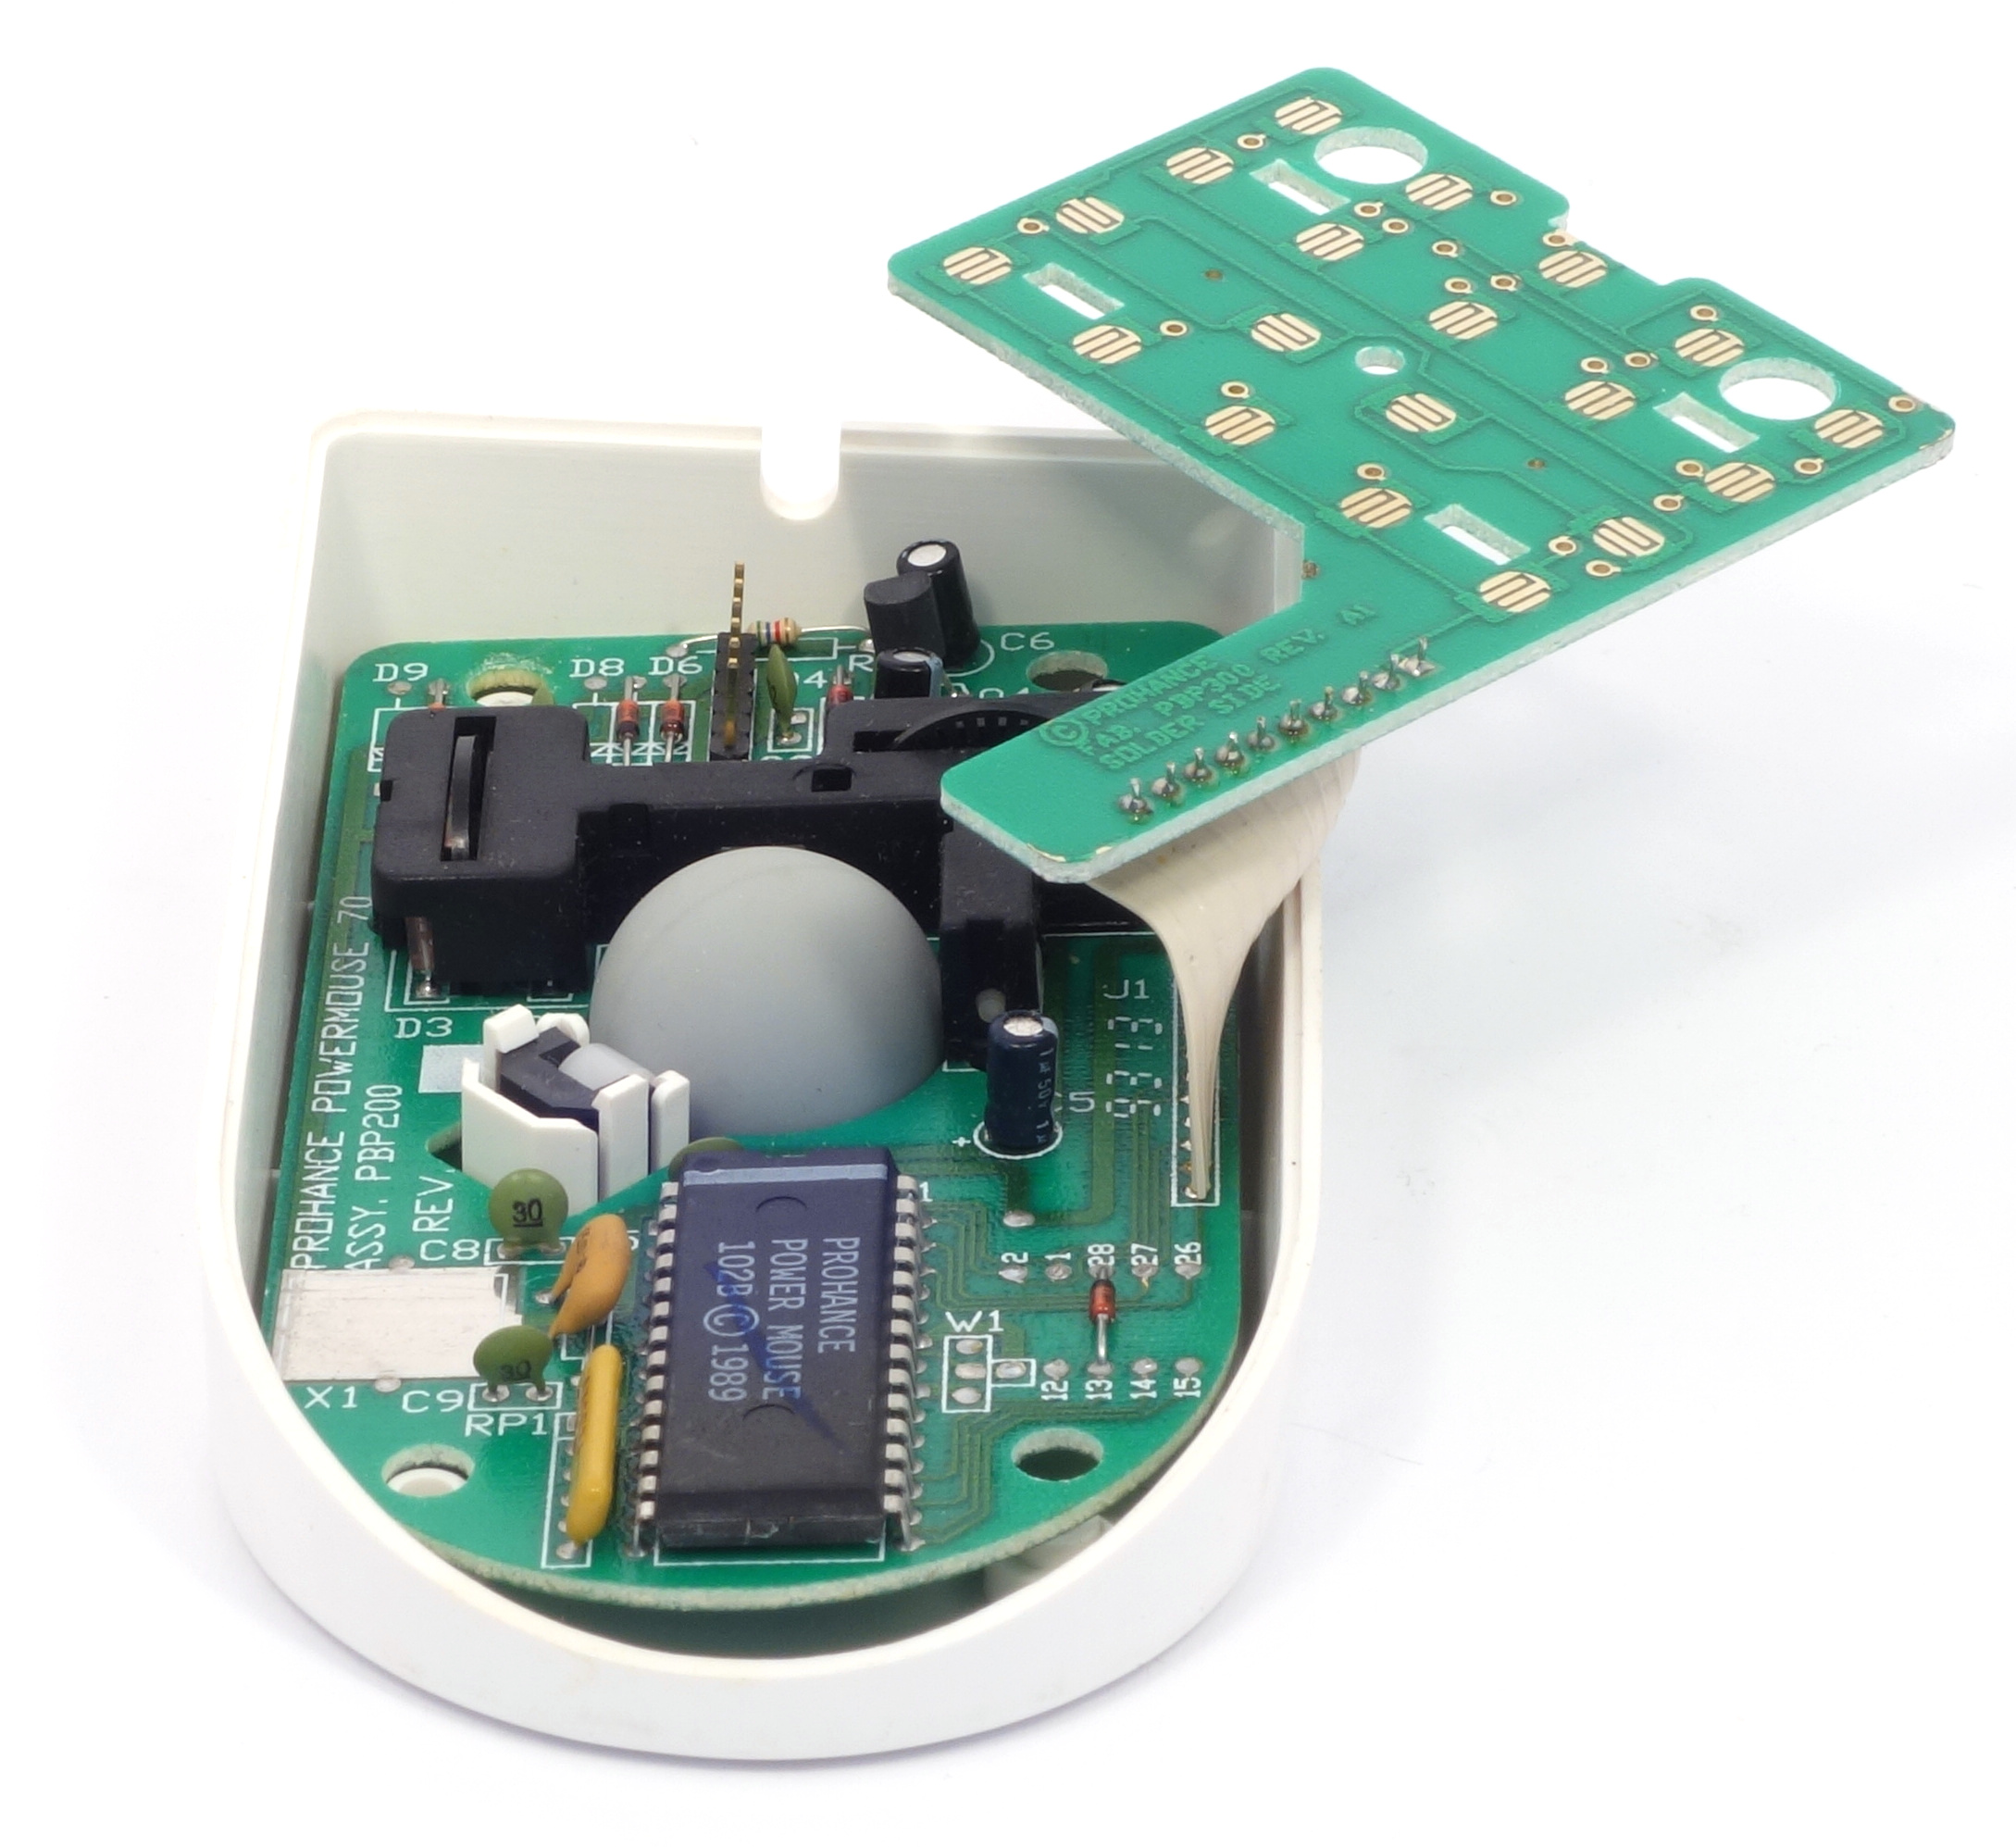
\includegraphics[scale=0.8]{1989_prohance_powermouse/inside_60.jpg}
    \caption{Prohance mouse disassembled}
    \label{fig:ProhanceInside}
\end{figure}

Mouse internals are shown on figure \ref{fig:ProhanceInside}. It is an opto-mechanical device typical for the beginning of the 90s, and the buttons and functional keys block is made on a separate printed circuit board: it is a miniature membrane keyboard similar to installed in pocket calculators. Also on the printed circuit board you can see the “Prohance Powermouse 70” text different from the number under which the model was on sale.

\begin{thebibliography}{9}
\bibitem{livingston} Livingston B. Genetically engineered mice run amok at Windows World // InfoWorld, Vol. 15, Iss. 21, May 24, 1989. - p. 34. \url{https://books.google.by/books?id=PTsEAAAAMBAJ&lpg=PA34&dq=prohance%20mouse&hl=ru&pg=PA34#v=onepage&q=prohance%20mouse&f=false}
\bibitem{prohance} Gruman G. What price mice? // Infoworld, V. 12, No. 17, April 23, 1990. - P. 63-69. \url{https://books.google.by/books?id=LTsEAAAAMBAJ&lpg=PA63&ots=GzwI8rKvl3&dq=%22prohance%20powermouse%22&pg=PA63#v=onepage&q&f=false}
\end{thebibliography}
\end{document}
